
\documentclass[11pt,a4paper]{ctexart}
\usepackage[utf8]{inputenc}
\usepackage{geometry}
\geometry{left=2.5cm,right=2.5cm,top=2.8cm,bottom=2.8cm}
\usepackage{amsmath,amssymb,amsfonts}
\usepackage{enumitem}
\usepackage{titlesec}
\usepackage{xcolor}
\usepackage{tcolorbox}
\usepackage{hyperref}

% 引入绝对位置放置宏包用于生成水印及插入图片宏包
\usepackage{graphicx}
\usepackage{eso-pic}

% 解决带圈数字在部分编译器下报错的问题


% --- 颜色定义 ---
\definecolor{mainblue}{RGB}{26, 82, 118}
\definecolor{secblue}{RGB}{41, 128, 185}
\definecolor{bglight}{RGB}{244, 246, 247}
\definecolor{textdark}{RGB}{44, 62, 80}

% --- 页面美化与字体设置 ---
\hypersetup{colorlinks=true, linkcolor=mainblue, urlcolor=secblue}
\setlist[itemize]{leftmargin=2em, itemsep=0.3em}
\setlist[enumerate]{leftmargin=2em, itemsep=0.3em}

% --- 标题样式自定义 ---
\titleformat{\section}{\large\bfseries\color{mainblue}}{\thesection}{1em}{}[{\color{mainblue}\titlerule[1pt]}]
\titleformat{\subsection}{\normalsize\bfseries\color{secblue}}{\thesubsection}{1em}{}
\titleformat{\subsubsection}{\small\bfseries\color{textdark}}{\thesubsubsection}{1em}{}

% --- 水印设置 (每页三个，斜45度，居中分布) ---
\newcommand{\WMText}{贺昱琪学习资料}
\newcommand{\WMScale}{2.28}
\newcommand{\WMAngle}{45}
\colorlet{WMColor}{black!8}

\AddToShipoutPictureBG{%
  \AtPageLowerLeft{%
    \put(\LenToUnit{0.66\paperwidth},\LenToUnit{0.70\paperheight}){%
      \rotatebox{\WMAngle}{\scalebox{\WMScale}{\textcolor{WMColor}{\WMText}}}%
    }%
    \put(\LenToUnit{0.33\paperwidth},\LenToUnit{0.50\paperheight}){%
      \rotatebox{\WMAngle}{\scalebox{\WMScale}{\textcolor{WMColor}{\WMText}}}%
    }%
    \put(\LenToUnit{0.66\paperwidth},\LenToUnit{0.30\paperheight}){%
      \rotatebox{\WMAngle}{\scalebox{\WMScale}{\textcolor{WMColor}{\WMText}}}%
    }%
  }%
}

\begin{document}

\begin{center}
    \LARGE \textbf{贺昱琪专项训练二}
\end{center}

\vspace{0.5cm}

\noindent \textbf{一、认真填一填（每小题 3 分，共 30 分）}

\begin{enumerate}
    \item $0.6$ 的倒数是\underline{\hspace{2cm}}。\vspace{1.2cm}
    
    \item 甲种蔬菜保鲜适宜的温度是 $1^\circ\text{C} \sim 5^\circ\text{C}$，乙种蔬菜保鲜适宜的温度是 $3^\circ\text{C} \sim 8^\circ\text{C}$，将这两种蔬菜放在一起同时保鲜，适宜的温度是\underline{\hspace{2cm}}。\vspace{1.2cm}
    
    \item 下边横排有 12 个方格，每个方格里填一个数，若任何相邻三个数的和都是 18，则 $x=$\underline{\hspace{2cm}}。\\
    \begin{center}
    \begin{tabular}{|c|c|c|c|c|c|c|c|c|c|c|c|}
        \hline
        5 & & & & & & $x$ & & & & & 10 \\
        \hline
    \end{tabular}
    \end{center}\vspace{1.2cm}
    
    \item 
    \begin{minipage}{0.65\textwidth}
        如图，将一圆盘四等分，并把四个区域分别标上I、II、III、IV，只有区域IV为感应区域。圆心角为 $65^\circ$ 的扇形 $AOB$ 绕点 $O$ 转动，在其半径 $OA$ 上装有带指示灯的感应装置，当扇形 $AOB$ 与区域IV有重叠（$O$点除外）的部分时，指示灯会发光；否则不发光。当扇形 $AOB$ 任意转动时，指示灯发光的可能性是\underline{\hspace{2cm}}。
    \end{minipage}
    \hfill
    \begin{minipage}{0.3\textwidth}
        \centering
        
\includegraphics[width=\linewidth]{4.png}
    \end{minipage}
    \vspace{1.2cm}
    
    \item 
    \begin{minipage}{0.65\textwidth}
        如图，将半径为 2cm 的圆形纸板沿着边长分别为 16cm 和 12cm 的长方形的外侧滚动一周并回到开始的位置，则圆心所经过的路线长为\underline{\hspace{2cm}}cm。（$\pi$取3）
    \end{minipage}
    \hfill
    \begin{minipage}{0.3\textwidth}
        \centering
        
\includegraphics[width=\linewidth]{5.png}
    \end{minipage}
    \vspace{1.2cm}
    
    \item 
    \begin{minipage}{0.65\textwidth}
        如图，把面积分别是 7 和 4 的两个正方形按如图所示拼在一起，其中 $B, C, E$ 三点在同一直线上，则图中阴影部分的面积为\underline{\hspace{2cm}}。
    \end{minipage}
    \hfill
    \begin{minipage}{0.3\textwidth}
        \centering
        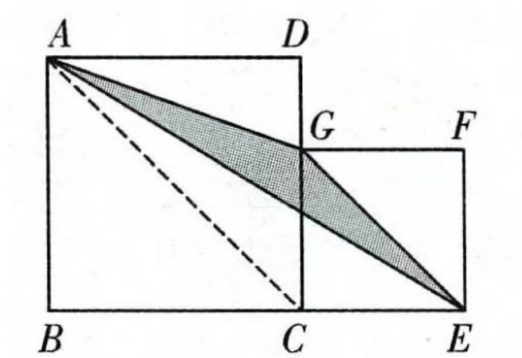
\includegraphics[width=\linewidth]{6.png}
    \end{minipage}
    \vspace{1.2cm}
    
    \item 在 $\triangle ABC$ 中，$BC=6$，$AC=3$，过点 $C$ 作 $CP \perp AB$，垂足为 $P$，则 $CP$ 长的最大值为\underline{\hspace{2cm}}。\vspace{1.2cm}
    
    \item 某会展中心大厅的 120 盏灯都是亮着的，每个灯都单独设有开关。现将开关按 $1 \sim 120$ 编号。小王同学先按下编号为 3 的倍数的开关，然后按下编号为 5 的倍数的开关。这时会展中心大厅中亮着的灯有\underline{\hspace{2cm}}盏。\vspace{1.2cm}
    
    \item 
    \begin{minipage}{0.65\textwidth}
        如图，“回”字形的道路宽为 1 米，整个“回”字形是一个长 16 米，宽 8 米的长方形场地。如果小丽沿着小路的中间从内部出发走完这条小路，那么她共走\underline{\hspace{2cm}}米。
    \end{minipage}
    \hfill
    \begin{minipage}{0.3\textwidth}
        \centering
        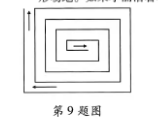
\includegraphics[width=\linewidth]{9.png}
    \end{minipage}
    \vspace{1.2cm}
    
    \item 
    \begin{minipage}{0.65\textwidth}
        如图，在由 6 个大小相同的正方形组成的方格中，设每个小正方形的边长均为 1。若连接三格和两格的对角线，则 $\angle \alpha + \angle \beta =$\underline{\hspace{2cm}}。
    \end{minipage}
    \hfill
    \begin{minipage}{0.3\textwidth}
        \centering
        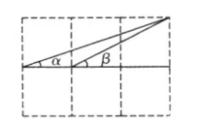
\includegraphics[width=\linewidth]{10.png}
    \end{minipage}
\end{enumerate}

\vspace{0.8cm}

\noindent \textbf{二、细心算一算（共 30 分）}

\begin{enumerate}
    \item[11.] 计算（每小题 5 分，共 20 分）
    \begin{enumerate}
        \item[(1)] $11\frac{7}{8} - 6\frac{1}{3} - 1\frac{1}{2}$
        \vspace{3.5cm}
        
        \item[(2)] $9\frac{2}{5} \div \left(2\frac{1}{4} \div 2\frac{1}{3} \times \frac{4}{5}\right)$
        \vspace{3.5cm}
        
        \item[(3)] $\left(\frac{7}{20} + \frac{1}{4} \times 60\%\right) \div \frac{7}{8} + \frac{8}{7}$
        \vspace{3.5cm}
        
        \item[(4)] $\left[ \frac{1}{7} + \left(0.75 - \frac{7}{20}\right) \div 7 \right] \times 3.5$
        \vspace{3.5cm}
    \end{enumerate}
    
    \item[12.] 解方程（每小题 5 分，共 10 分）
    \begin{enumerate}
        \item[(1)] $\frac{3}{4}x - 2 = x$
        \vspace{3.5cm}
        
        \item[(2)] $\frac{1}{3}(2x - 1) - \frac{x+2}{6} = 1$
        \vspace{3.5cm}
    \end{enumerate}
\end{enumerate}

\vspace{0.8cm}

\noindent \textbf{三、用心想一想（共 28 分）}

\begin{enumerate}
    \item[13.] (8分) 
    \begin{minipage}{0.65\textwidth}
        某学校为了丰富学生课余生活，开展了“第二课堂”活动，推出了以下五种选修课程：$A$. 绘画；$B$. 唱歌；$C$. 跳舞；$D$. 演讲；$E$. 书法。学校规定：每个学生都必须报名且只能选择其中的一个课程。学校随机抽查了部分学生，对他们选择的课程情况进行了统计，并绘制了如下两幅不完整的统计图。请结合统计图中的信息解决下列问题：
        \begin{enumerate}
            \item[(1)] 这次抽查的学生人数是\underline{\hspace{2cm}}人；
            \item[(2)] 将条形统计图补充完整；
            \item[(3)] 扇形统计图中课程 $E$ 所对应的扇形的圆心角的度数是\underline{\hspace{2cm}}度；
            \item[(4)] 如果该校共有 1200 名学生，请你估计该校选择课程 $D$ 的学生约有多少人？
        \end{enumerate}
    \end{minipage}
    \hfill
    \begin{minipage}{0.3\textwidth}
        \centering
        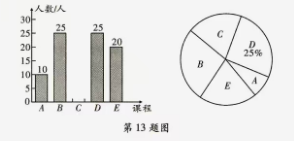
\includegraphics[width=\linewidth]{13.png}
    \end{minipage}
    \vspace{1.5cm}

    \item[14.] (10分) 如图，$A, B$ 两地相距 200km。其间一处因山体滑坡导致连接这两地的公路受阻。甲、乙两个工程队接到指令，要求于早上 8 点整分别从 $A, B$ 两地同时出发赶往滑坡点疏通公路。上午 10 点整甲队赶到并立即开始作业，半个小时后乙队赶到，并迅速投入“战斗”与甲队共同作业。此时甲队已完成了工程量的 $\frac{1}{6}$。
    
    \begin{center}
        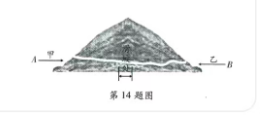
\includegraphics[width=0.45\textwidth]{14.png}
    \end{center}
    
    \begin{enumerate}
        \item[(1)] 若滑坡受阻公路长为 14km，甲队赶往滑坡点的速度是乙队的 1.5 倍少 5km，求乙队赶路的速度是多少？
        \vspace{4.0cm}
        
        \item[(2)] 如果下午 5 点整，两队完成公路疏通任务并顺利会师，那么乙工程队单独疏通这段公路需要多少小时？
        \vspace{4.0cm}
    \end{enumerate}
    
    \item[15.] (10分) 七年级数学兴趣小组准备了一个无盖的圆柱体容器和若干个 $A, B$ 两种型号的钢球。先往容器里加入一定量的水，水面高度为 40mm（如图）。水足以淹没所有的钢球，下面探究过程中水的损耗忽略不计。
    
    \begin{center}
        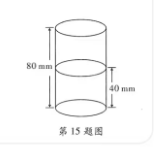
\includegraphics[width=0.35\textwidth]{15.png}
    \end{center}
    
    \noindent \textbf{探究一：}\\
    小组做了两次实验，先放入 3 个 $A$ 型号钢球，水面的高度上升了 12mm；把 3 个 $A$ 型号钢球捞出，再放入 4 个 $B$ 型号钢球，水面的高度恰好也上升了 12mm。由此可得一个 $A$ 型号钢球可以使水位上升\underline{\hspace{2cm}}mm，一个 $B$ 型号钢球可以使水位上升\underline{\hspace{2cm}}mm；
    \vspace{2.0cm}
    
    \noindent \textbf{探究二：}\\
    小组把之前的钢球全部捞出，然后再放入 $A$ 型号与 $B$ 型号钢球共 10 个后，水面高度达到 72mm，求放入水中的 $A$ 型号与 $B$ 型号钢球各几个？
    \vspace{4.0cm}
    
    \noindent \textbf{探究三：}\\
    小组把之前的钢球全部捞出，然后再放入 $A$ 型号与 $B$ 型号钢球共 $a$ 个，此时水面高度刚好达到 80mm（水未溢出）。求当 $a$ 最大时，放入水中的 $A$ 型号与 $B$ 型号钢球各几个？并求出 $a$ 的最大值。
    \vspace{4.5cm}
\end{enumerate}

\vspace{0.8cm}

\noindent \textbf{四、勇敢闯一闯（共 12 分）}

\begin{enumerate}
    \item[16.] (12分) 
    \begin{minipage}{0.65\textwidth}
        如图①，在长方形 $ABCD$ 中，$AB=30\text{cm}$，$BC=60\text{cm}$。点 $P$ 从点 $A$ 出发，沿 $A \rightarrow B \rightarrow C \rightarrow D$ 路线向点 $D$ 匀速运动，到达点 $D$ 后停止；点 $Q$ 从点 $D$ 出发，沿 $D \rightarrow C \rightarrow B \rightarrow A$ 路线向点 $A$ 匀速运动，到达点 $A$ 后停止。若点 $P, Q$ 同时出发，在运动过程中，$Q$ 点停留了 1 秒，图②是 $P, Q$ 两点在折线 $AB-BC-CD$ 上相距的路程 $S$ (cm) 与时间 $t$ (秒) 之间的关系图象。解决下列问题：
        \begin{enumerate}
            \item[(1)] 点 $P$ 的运动速度是\underline{\hspace{2cm}}cm/s，点 $Q$ 的运动速度是\underline{\hspace{2cm}}cm/s；
            \item[(2)] 点 $Q$ 到达点 $A$ 所需时间为\underline{\hspace{2cm}}秒；
            \item[(3)] 若 $\triangle PCQ$ 为等腰三角形，则 $t$ 的值为\underline{\hspace{4cm}}。
        \end{enumerate}
    \end{minipage}
    \hfill
    \begin{minipage}{0.3\textwidth}
        \centering
        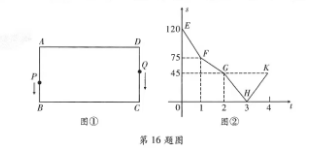
\includegraphics[width=\linewidth]{16.png}
    \end{minipage}
    \vspace{4.5cm}
\end{enumerate}

\end{document}

